\documentclass{beamer}
\usepackage{graphicx}
\usepackage{bibentry}

\title{Logical structure extraction from scanned documents}
\author{Bogatenkova A.O., Kozlov I.S., Belyaeva O.V., Perminov A.I.}
\date{September 25, 2020}


\setbeamertemplate{footline}[frame number]

\begin{document}

\begin{frame}
\titlepage
\end{frame}

\begin{frame}{Introduction}
    A huge number of scanned documents exist that one needs to work with. Extraction the structure from such documents may be useful for their analysis.
    \hspace{0.5cm}
    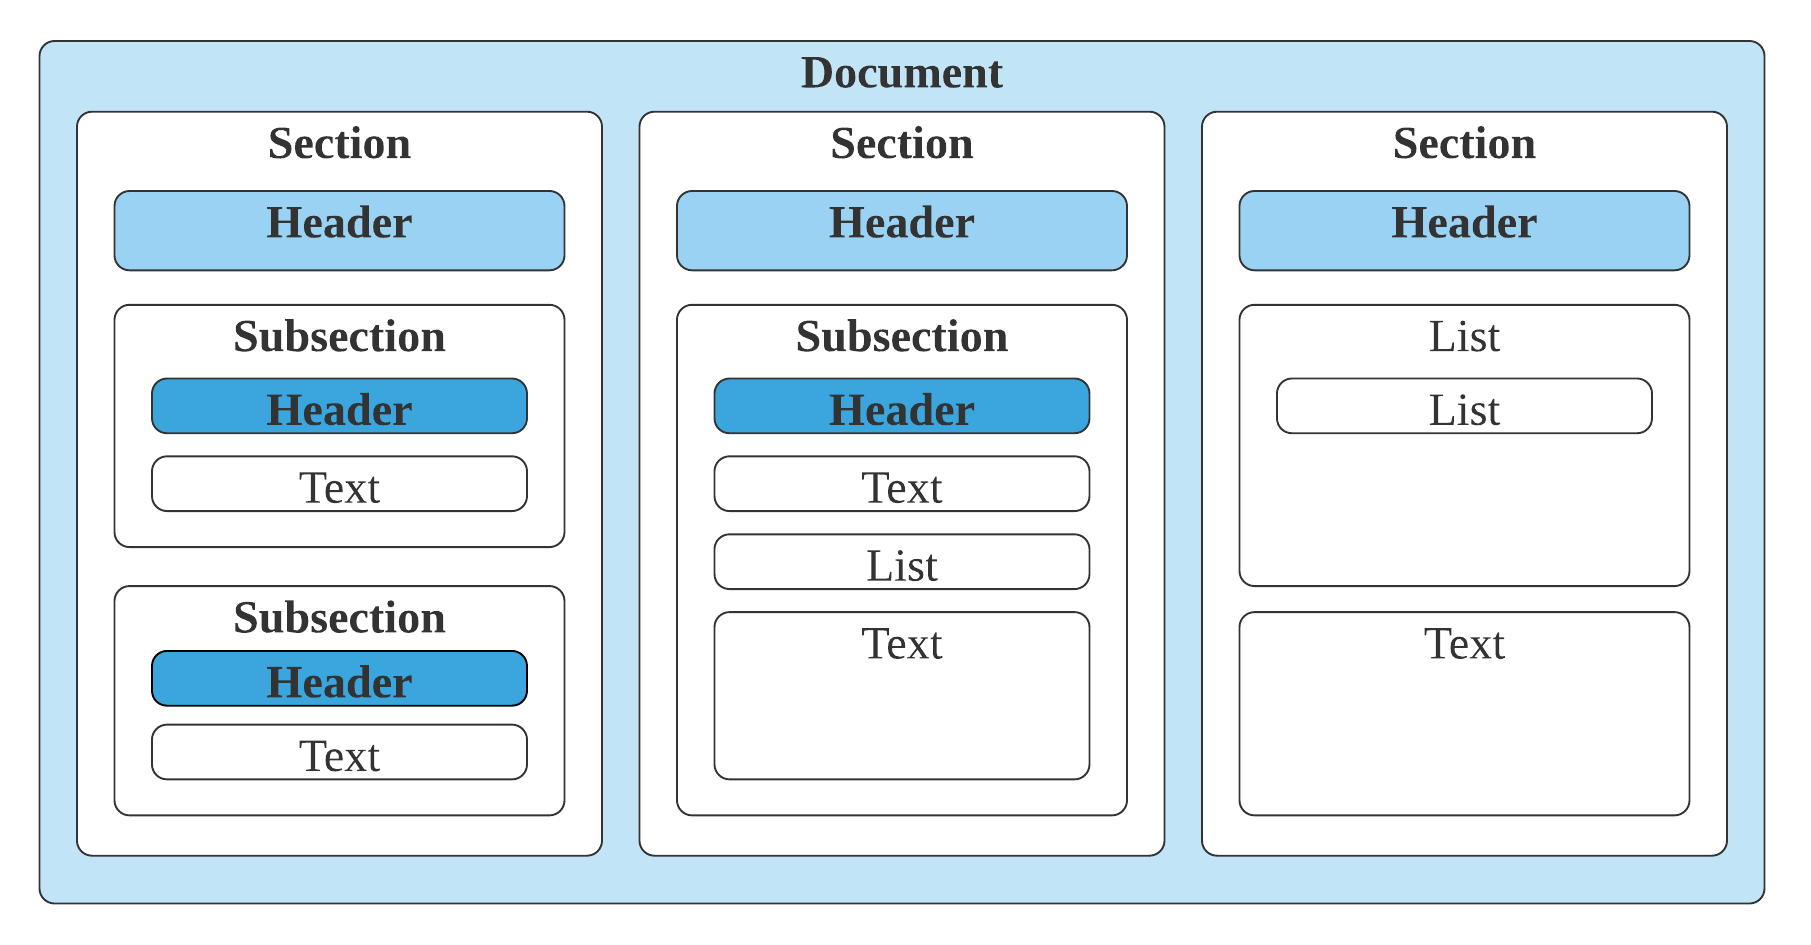
\includegraphics[width=\textwidth]{pics/structure.png}
\end{frame}

\begin{frame}{The purpose of the work}
    The task of extracting a logical structure from documents is being solved. We will describe the pipeline for scanned documents processing. The method is based on the multiclass classification of document lines. The set of classes includes:
    \begin{itemize}
        \item headers;
        \item list elements;
        \item textual lines.
    \end{itemize}
    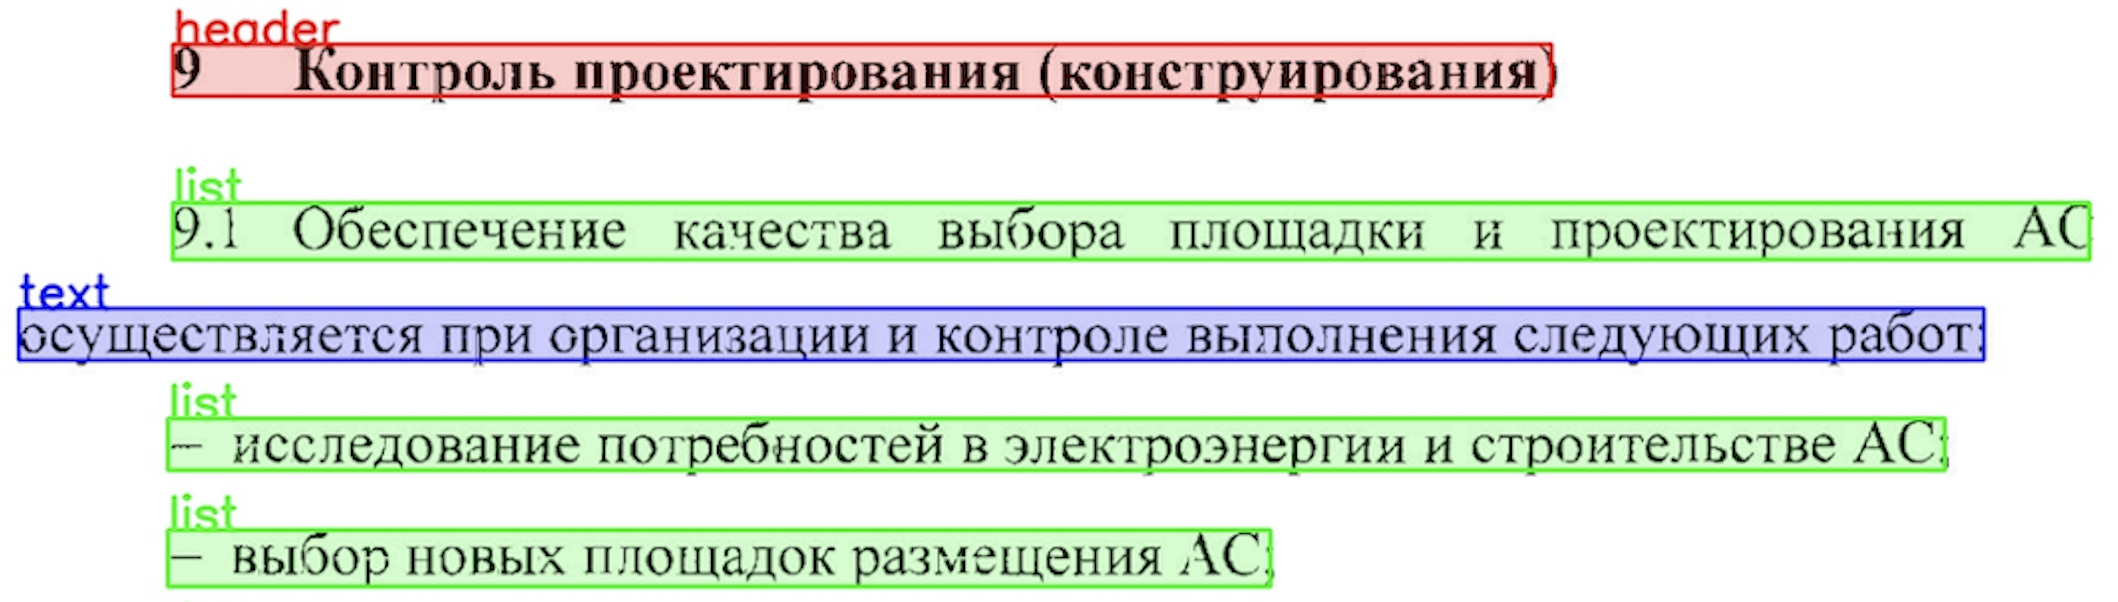
\includegraphics[width=\textwidth]{pics/structure_example.png}
\end{frame}

\begin{frame}{Related work}
    Several approaches for structure extraction from documents exist:
    \begin{itemize}
        \item methods based on table of contents (TOC);
        \item rule based methods;
        \item methods based on machine learning.
    \end{itemize}
\end{frame}

\begin{frame}{1. Structure extraction using table of contents}
    \begin{columns}
        \begin{column}{0.5\textwidth}
        A lot of ICDAR competitions connected with the analysis of documents are held. In one of these competitions, the structure was extracted from books. It was proposed that books consist of pages, paragraphs, chapters, such structure was extracted using the table of contents, which was present in most books.
        \end{column}
        \begin{column}{0.5\textwidth}
        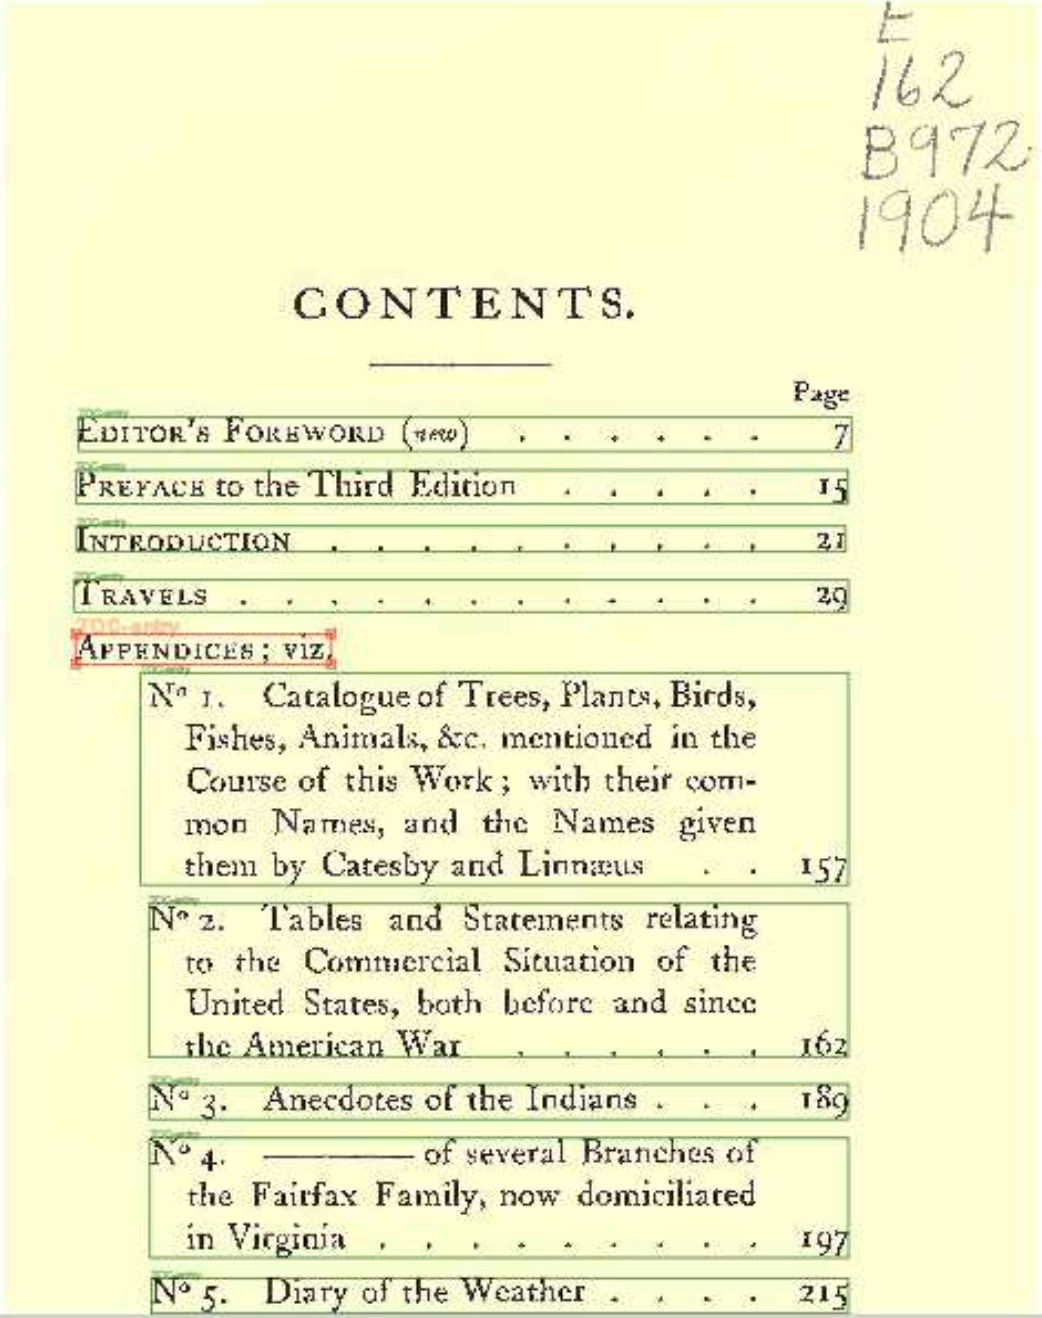
\includegraphics[width=\textwidth]{pics/toc.png}
        \end{column}
    \end{columns}
\end{frame}

\begin{frame}{2. Rule based methods}
    \begin{columns}
        \begin{column}{0.5\textwidth}
        In 2019 on the FinTOC competitions a structure was extracted from financial documents in the form of a hierarchy of document headings with different levels.
        
        One of the participating teams extracted the necessary structure using the table of contents and rules (line spacing, indentation, font, numbering).
        \end{column}
        \begin{column}{0.5\textwidth}
        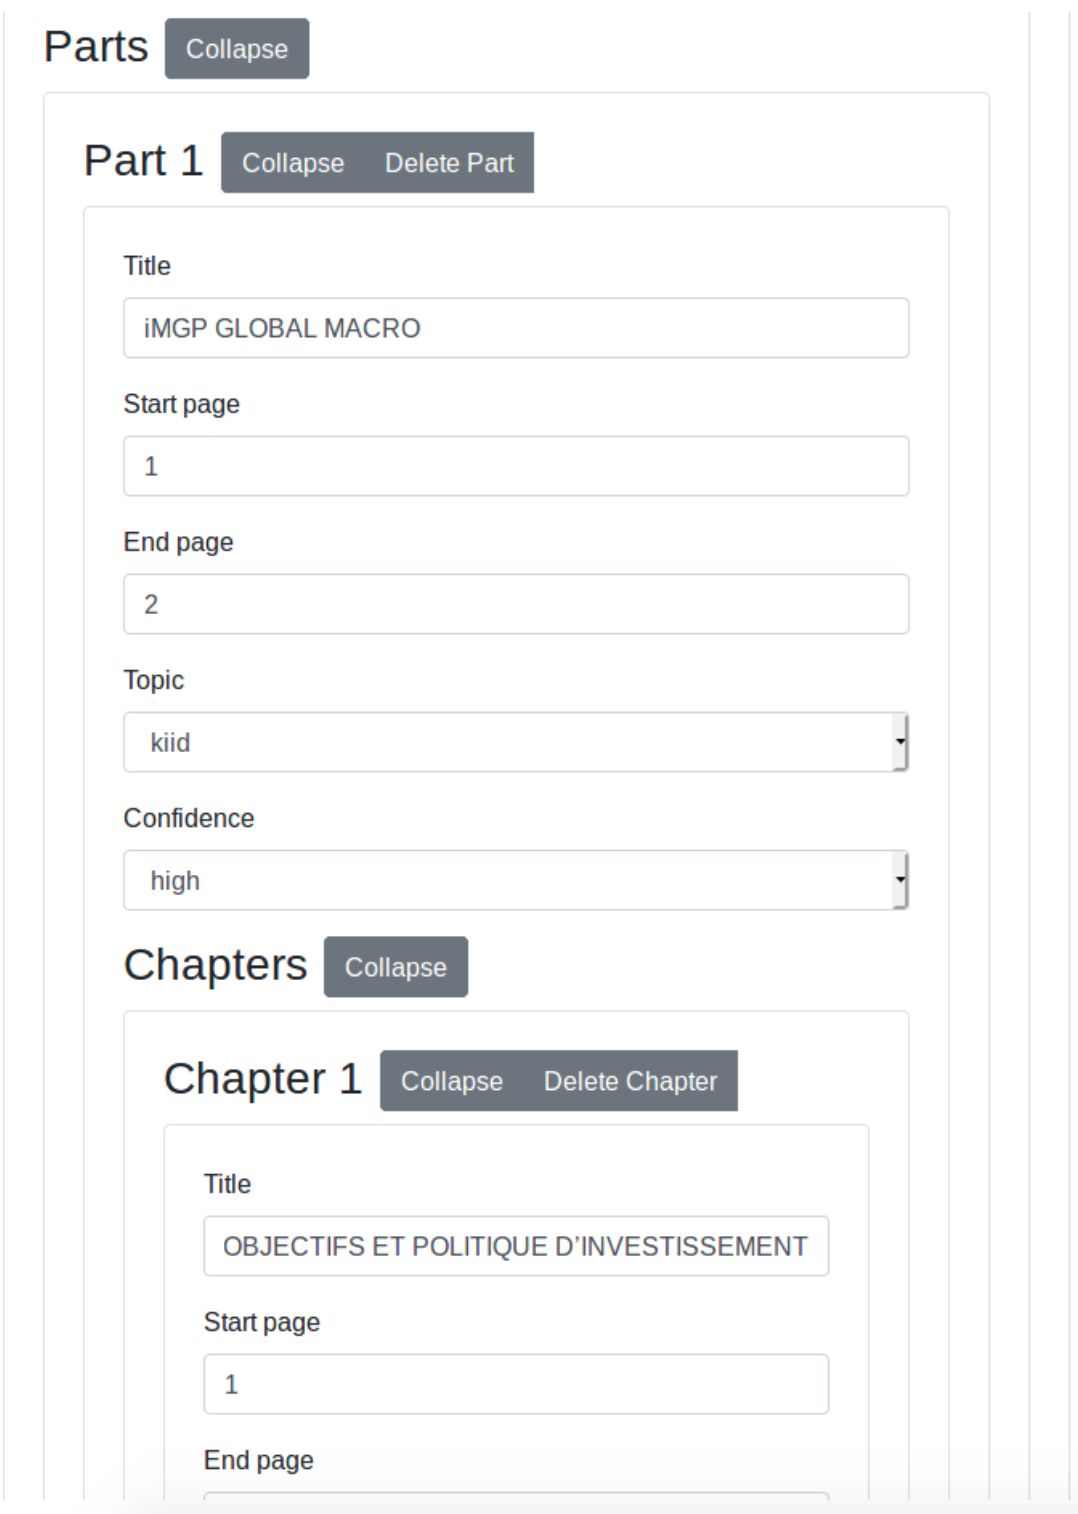
\includegraphics[width=\textwidth]{pics/rulebased.png}
        \end{column}
    \end{columns}
\end{frame}

\begin{frame}{3. Methods based on machine learning.}
% TODO links
        In a 2017 article, document structure was extracted using machine learning techniques including deep learning. Firstly, the classifier for lines determined if the line was the title or not, then the title lines were classified more precisely by section classifiers.
        
        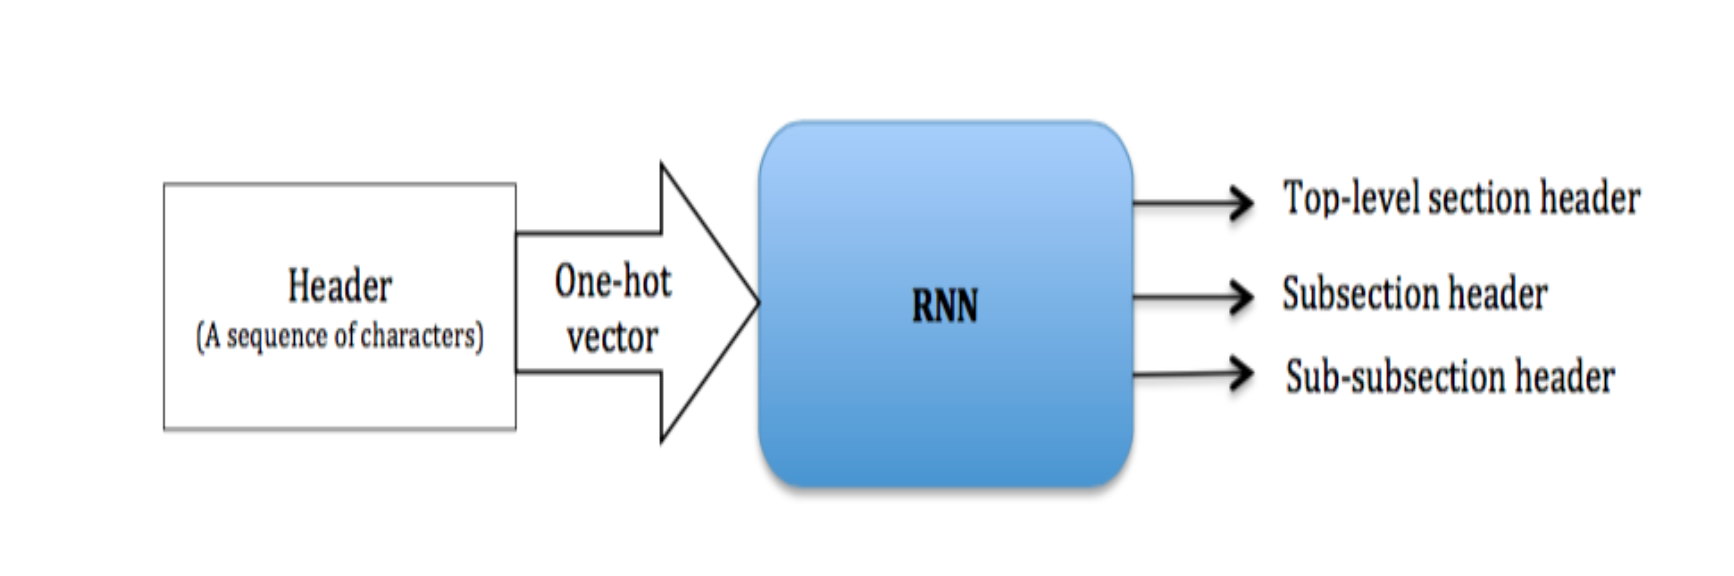
\includegraphics[width=\textwidth]{pics/classifier.png}
\end{frame}

\begin{frame}{Difficulties in using existing solutions}
\begin{itemize}
    \item Documents can contain deeply nested headings or numbered list items.
    \item As a rule, existing solutions are focused on the extraction of the hierarchy of headers, for our task it is also necessary to extract the elements of the lists.
    \item In most of the examples given above, the classification of text blocks is carried out, in our task, we should classify each line of the document.
\end{itemize}
\end{frame}

\begin{frame}{Dataset description}
    \begin{columns}
        \begin{column}{0.5\textwidth}
        The dataset is a collection of document JPEG images downloaded from zakupki.gov.ru. The images are scanned copies of government procurements documents. Each image considered as a separate document. The dataset didn't include documents containing tables, figures, frames and other non-text elements.
        \end{column}
        \begin{column}{0.5\textwidth}
        \frame{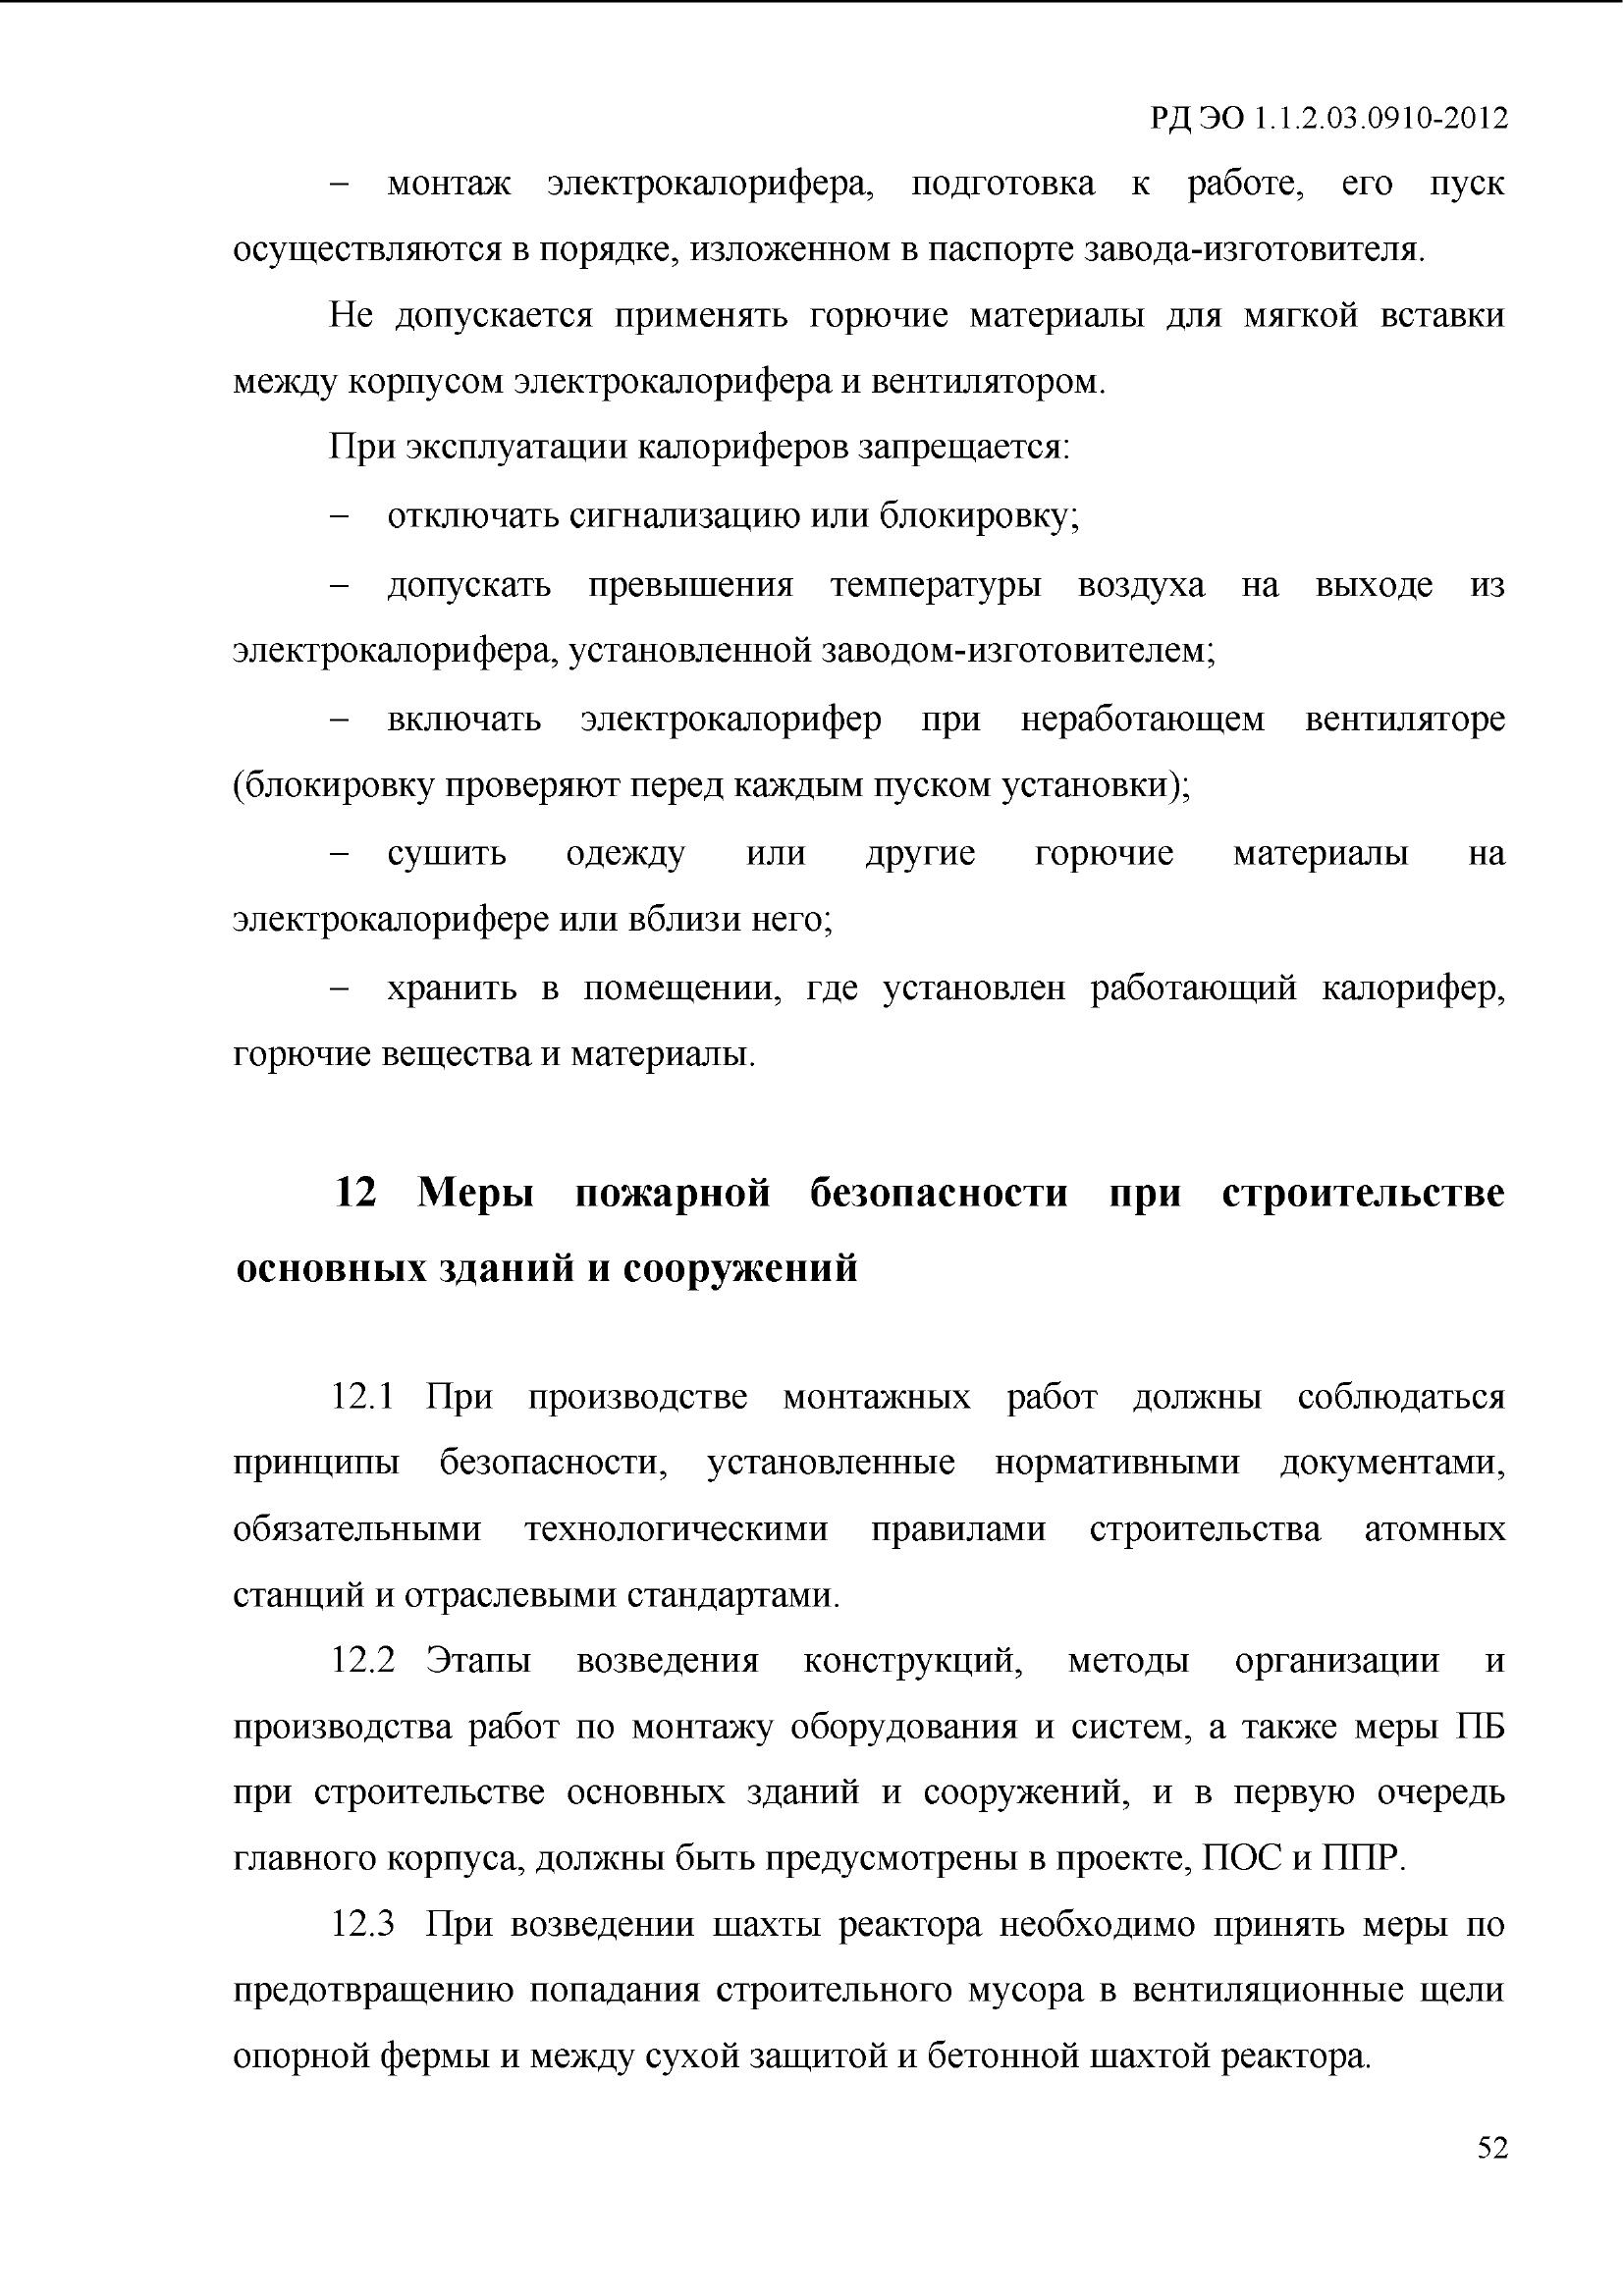
\includegraphics[width=\textwidth]{pics/doc_example.jpeg}}
        \end{column}
    \end{columns}
\end{frame}

\begin{frame}{Data labelling}
    The process of creating labeled data includes the following steps:
    \center{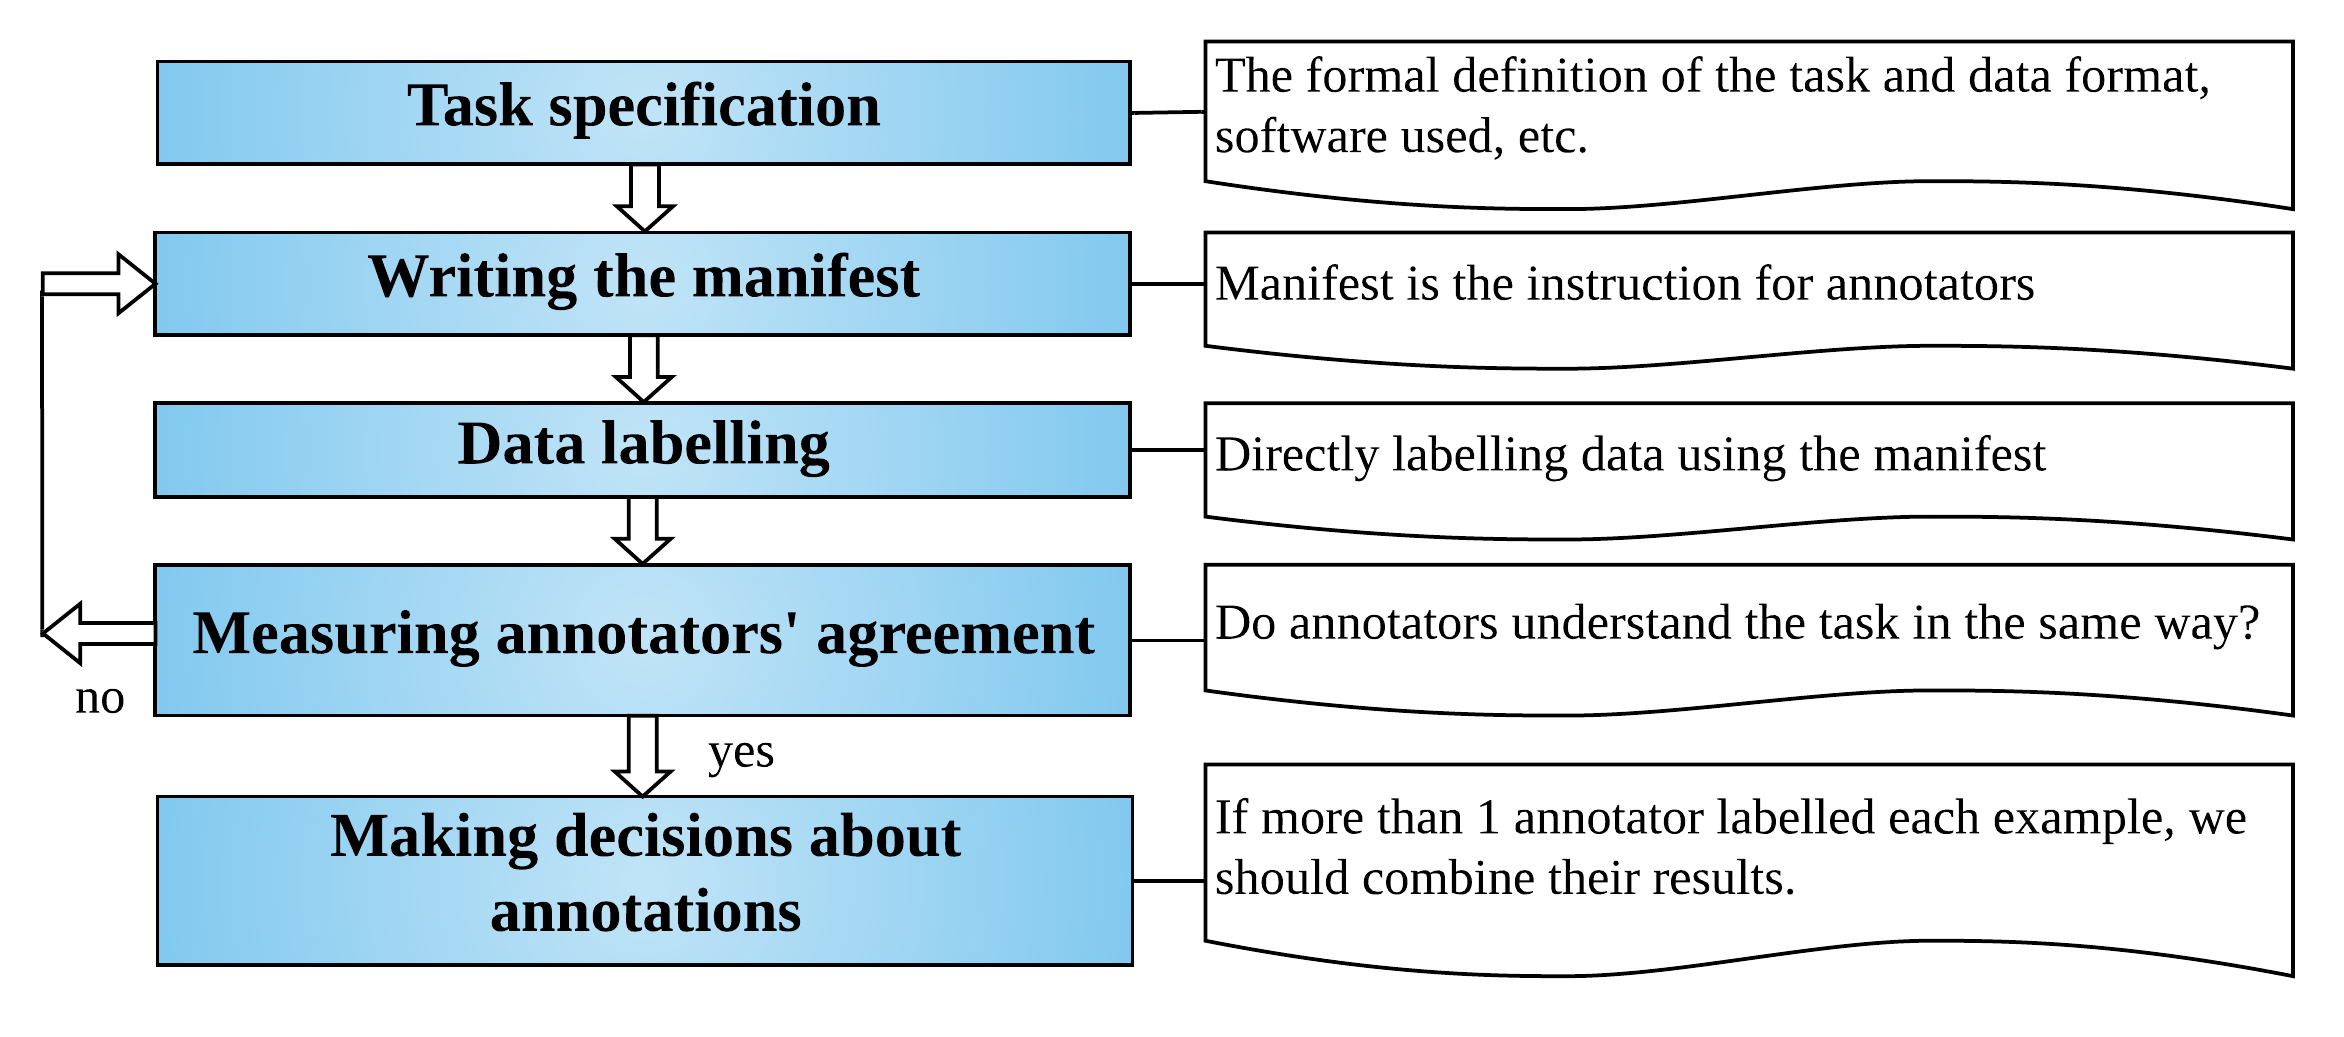
\includegraphics[width=\textwidth]{pics/labelling.png}}
\end{frame}

\begin{frame}{Task specification}
    Our task is a multiclass classification of document lines. The images of the scanned document with the next line for labelling outlined in a blue frame were sequentially shown to annotators. Annotators should assign the text in the frame to one of the predefined classes: 
    \begin{itemize}
        \item header;
        \item list item;
        \item text;
        \item other.
    \end{itemize}
\end{frame}

\begin{frame}{The manifest}
    \begin{columns}
        \begin{column}{0.45\textwidth}
        To define the labelling rules for annotators, the manifest has been developed. It contains formal rules for classifying document lines.
        \end{column}
        \begin{column}{0.55\textwidth}
        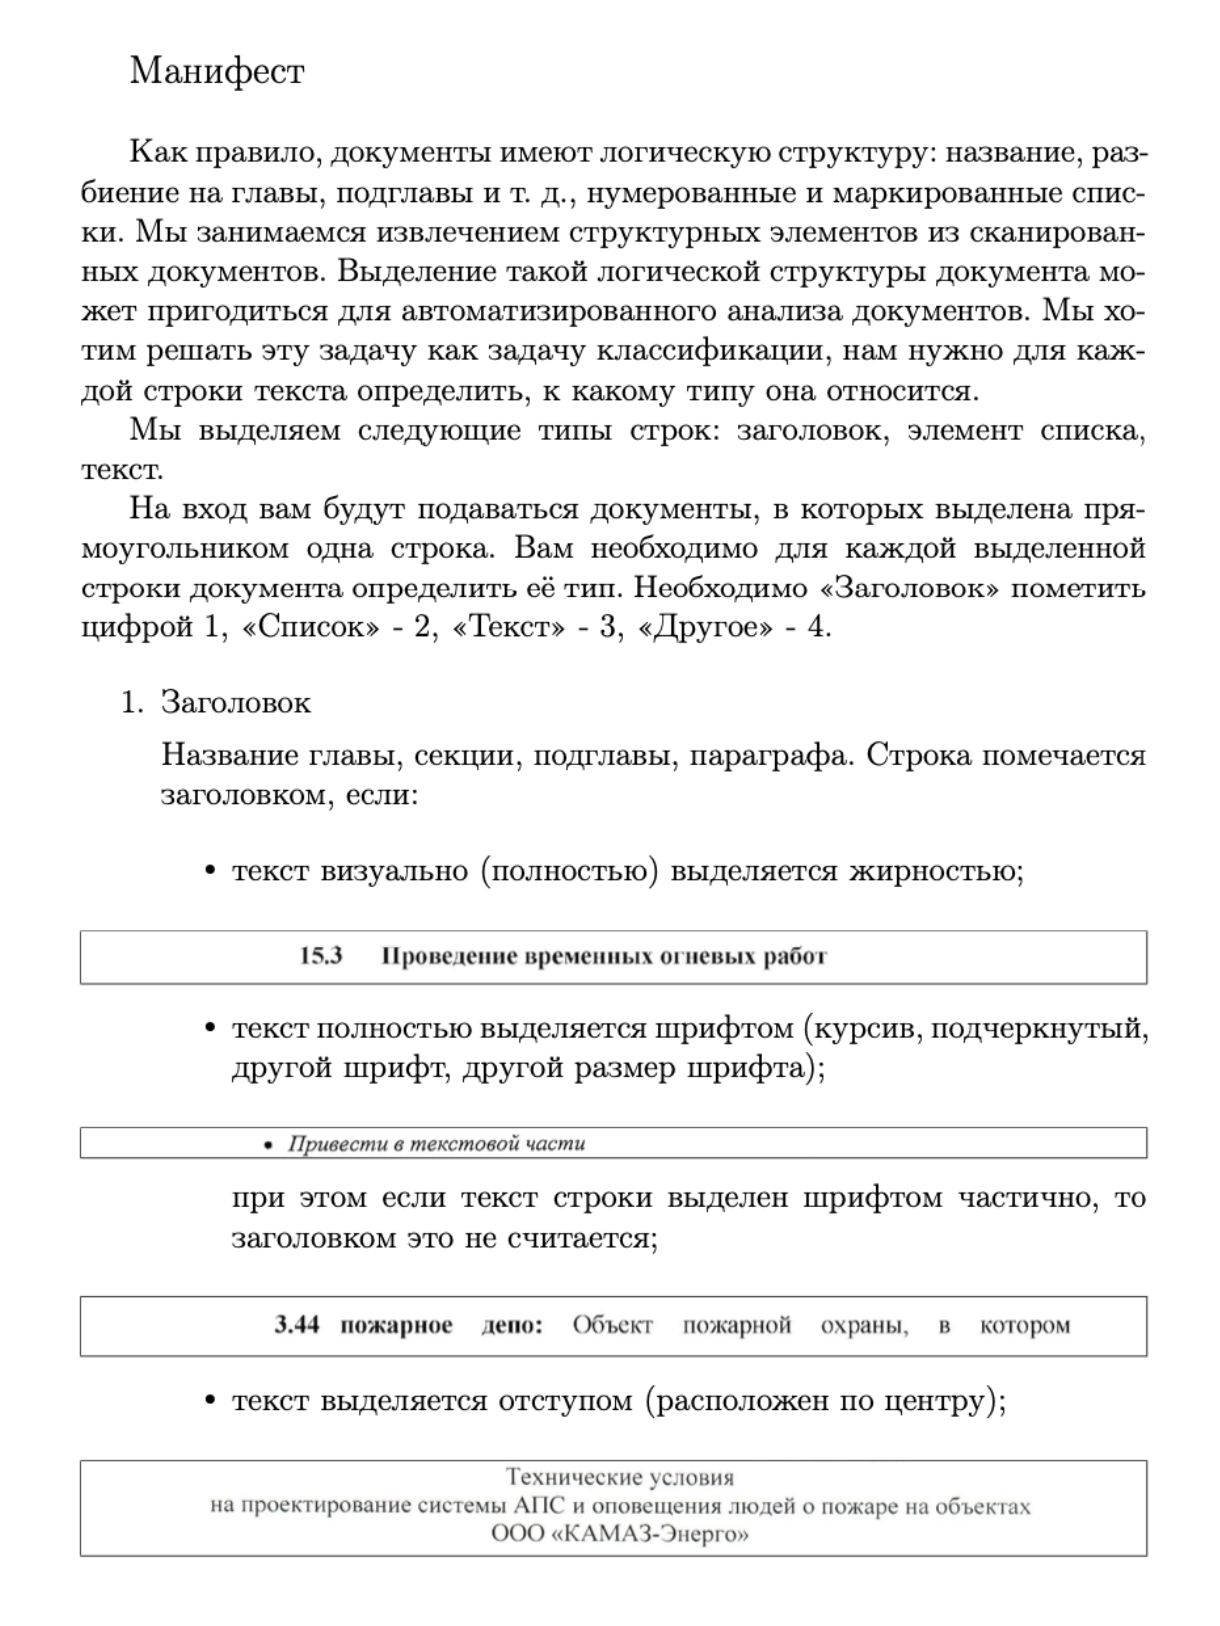
\includegraphics[width=\textwidth]{pics/manifest.png}
        \end{column}
    \end{columns}
\end{frame}

\begin{frame}{Data labelling}
    The proprietary system was used for the annotation process.
    \frame{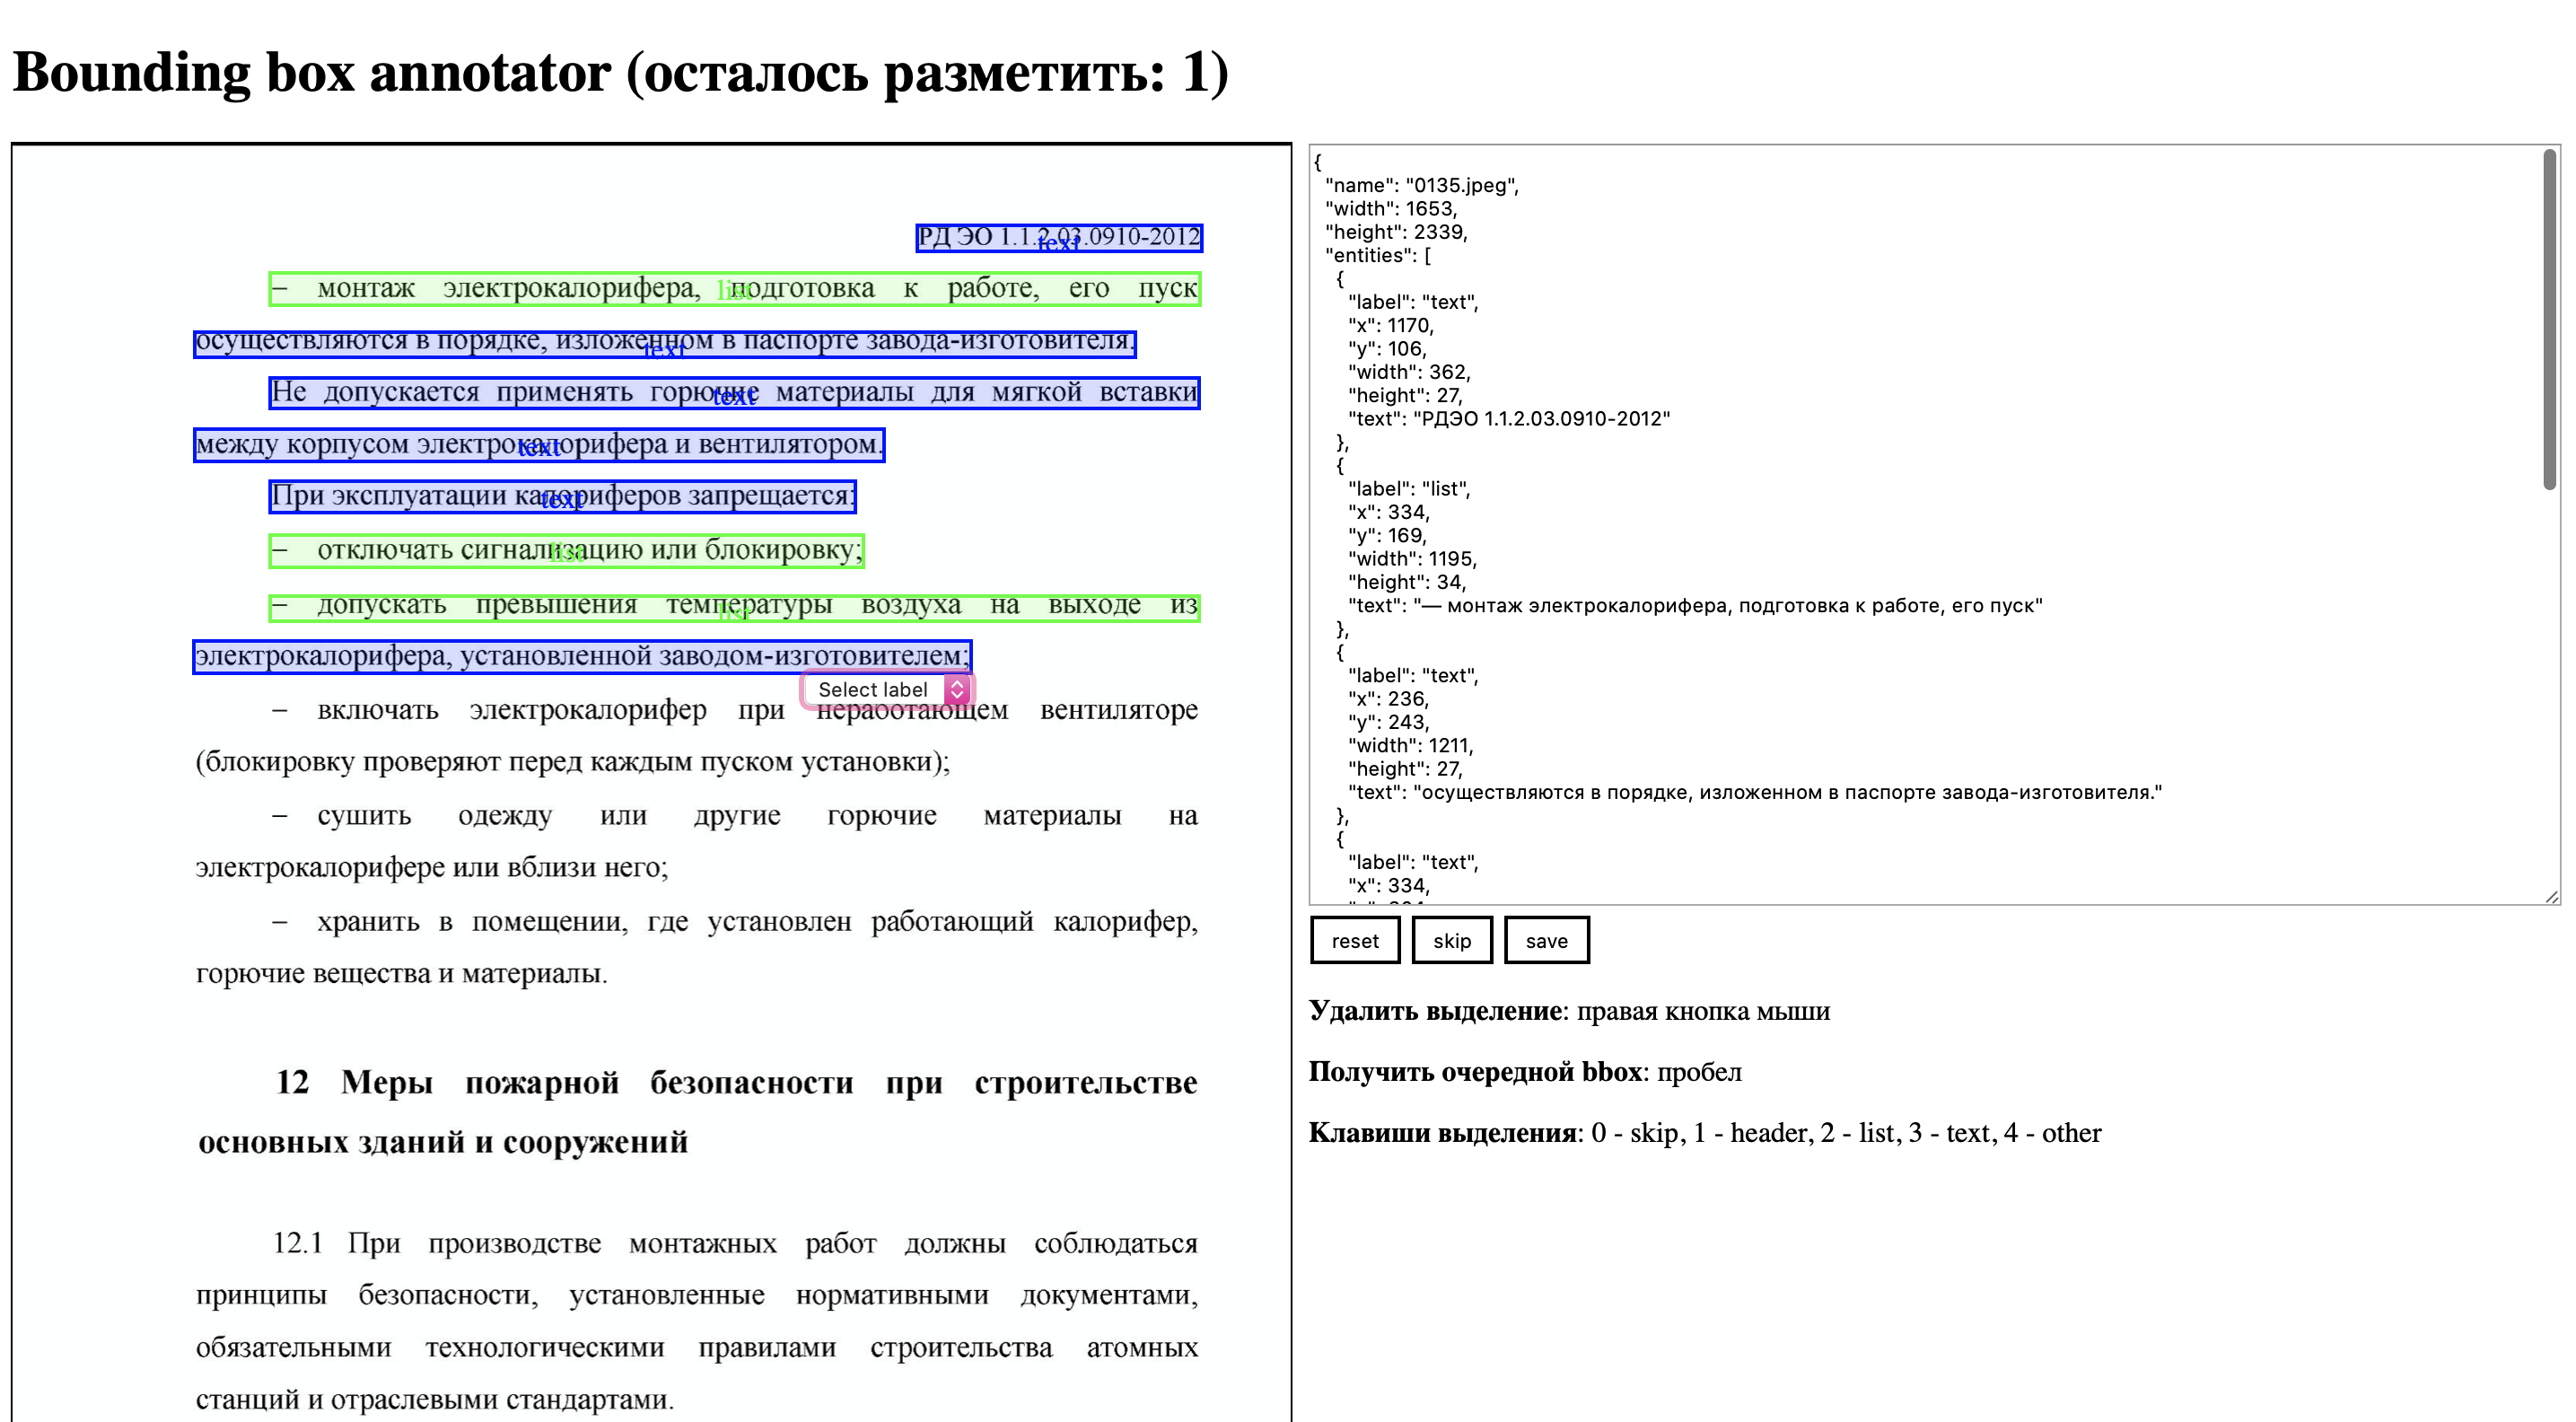
\includegraphics[width=\textwidth]{pics/annotation.png}}
\end{frame}

\begin{frame}{Annotators' agreement}
    Cohen's kappa $\kappa$ statistic was calculated to check the correctness of the labelling.
    $$ \kappa = \frac{p_o-p_e}{1-p_e}, \kappa \leq 1 $$
    $p_o$ - the relative observed agreement among raters (accuracy);
    
    $p_e$ - the hypothetical probability of chance agreement.
    
    The closer $\kappa$ is to 1, the higher the agreement between annotators. After labelling 10 documents (407 lines) by two annotators, the value of the $\kappa$ statistic was 0.975, which is considered as a high level of agreement. 
    
    Then  600 documents (21350 lines) were labelled.
\end{frame}

\begin{frame}{Method description}
    Pipeline for documents processing:
    \center{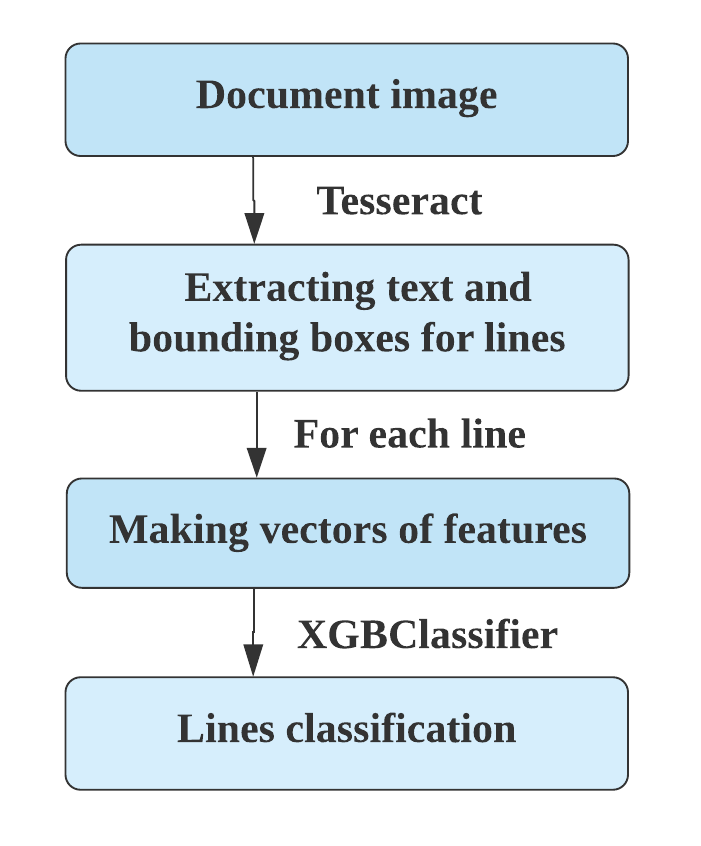
\includegraphics[width=0.5\textwidth]{pics/pipeline.png}}
\end{frame}

\begin{frame}{Feature extraction}
    3 types of features were extracted:
    \begin{itemize}
        \item \textbf{Regular expression-based features} (the line starts with an uppercase or lowercase letter, number, dash, etc., the line ends with a letter, period or semicolon).
        \item \textbf{Textual features} (number of letters in the first word, line length, number of words in a line).
        \item \textbf{Visual features} (left indentation, font weight, text height).
    \end{itemize}
    In addition, the features of the four previous (subsequent) lines and the average values of some features were used.
\end{frame}

\begin{frame}{Classifier selection}
    \center{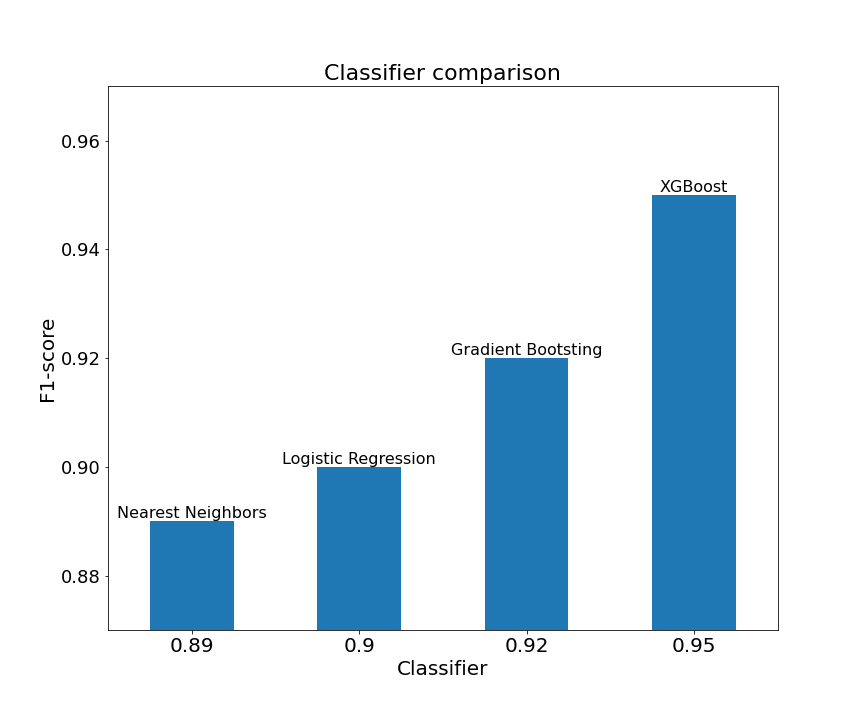
\includegraphics[width=0.9\textwidth, height=8cm]{pics/scores.png}}
\end{frame}

\begin{frame}{Features' importances analysis}
    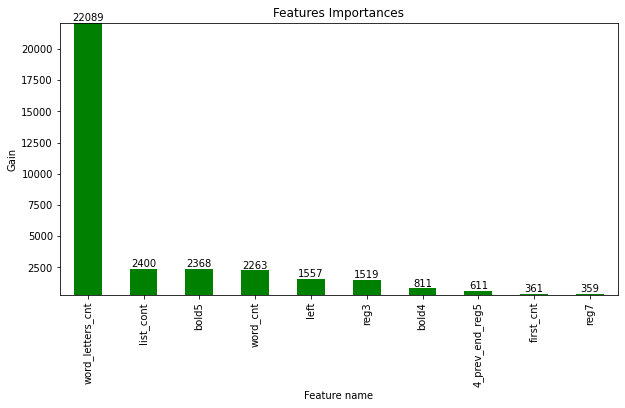
\includegraphics[width=\textwidth]{pics/gaines.png}
\end{frame}

\begin{frame}{Results}
    \begin{itemize}
        \item XGBClassifier parameters after model tuning:
        $learning\_rate = 0.1$
    
        $n\_estimators = 1000$
        
        $max\_depth = 7$
        
        $min\_child\_weight = 2$
        
        $gamma = 0$
        
        $subsample = 1$
        
        $colsample\_bytree = 1$
        
        $alpha = 0.01$
        \item F1-score on the cross-validation: 
        $0.98995$.
    \end{itemize}
\end{frame}

\begin{frame}{Errors analysis}
    \center{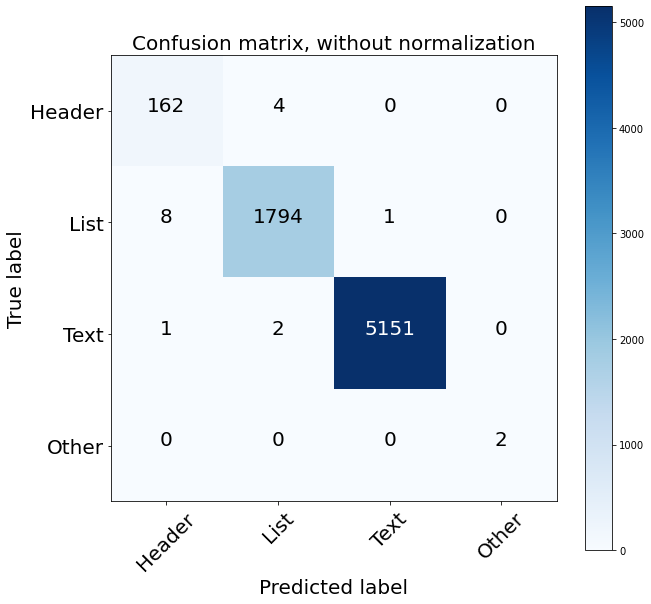
\includegraphics[width=0.8\textwidth, height=7.5cm]{pics/conf_matrix.png}}
\end{frame}

\begin{frame}{Conclusion}
    \begin{enumerate}
        \item The method for extracting the logical structure based on the classification of document lines is developed.
        \item The pipeline is implemented, consisting of processing documents using the Tesseract program for extracting lines and bounding boxes, making feature vectors and training the classifier.
        \item The dataset obtained using manual labelling is available.
    \end{enumerate}
\end{frame}

\end{document}